\documentclass[a4paper,11pt]{article}

% --- Packages ---
\usepackage[utf8]{inputenc}
\usepackage[T1]{fontenc}
\usepackage{geometry}
\usepackage{graphicx}
\usepackage{svg}
\usepackage{booktabs}
\usepackage{tabularx}
\usepackage{siunitx}
\usepackage{amsmath}
\usepackage{amssymb}
\usepackage{hyperref}
\usepackage{caption}
\usepackage{fancyhdr}
\usepackage{subcaption}
\usepackage{float}
\usepackage{scrextend}
\usepackage[style=ieee, backend=biber]{biblatex}

% --- Configuration ---
\geometry{top=2.5cm, bottom=2.5cm, left=2.5cm, right=2.5cm}

\addbibresource{references.bib}

\sisetup{
    output-decimal-marker = {.},
    group-digits = true,
    per-mode = symbol
}

% SVG Settings
% DO NOT use \svgsetup{convert=true} with the standard 'svg' package.
% Just ensure Inkscape is in PATH and compile with --shell-escape.
% The 'svg' package will automatically call Inkscape to convert .svg to .pdf.

\hypersetup{
    colorlinks=true,
    linkcolor=blue,
    filecolor=magenta,      
    urlcolor=cyan,
    pdftitle={HumanEd: Mo6},
    pdfauthor={Benjamin McEwan}
}

% --- DOCUMENT -------------------------------------------------------------------------------------
\begin{document}

\title{\textbf{HumanEd: Mo-6 "Morris" 6-Axis Serial Manipulator}}
\author{Benjamin McEwan}
\date{\today}
\maketitle

\tableofcontents


% --- OVERVIEW -------------------------------------------------------------------------------------
\newpage
\section{Overview}\label{sec:overview}
% \begin{figure}[h!]
%     \centering
%     \includegraphics[width=0.5\linewidth]{img/mockup_shell.png} 
%     \caption{Mockup of Oar}
%     \label{fig:mockup}
% \end{figure}

The Mo-6 robot has been designed as a low-cost 6-axis serial manipulator that can be easily tailored to use different control systems and end-effectors. The robot follows the standard joint arrangement seen on many industrial 6-DOF manipulators, with a 2R open-chain attached to a rotating base used as the positioning system for a spherical wrist.

\subsection{Kinematics}
\begin{figure}[h!]
    \centering
    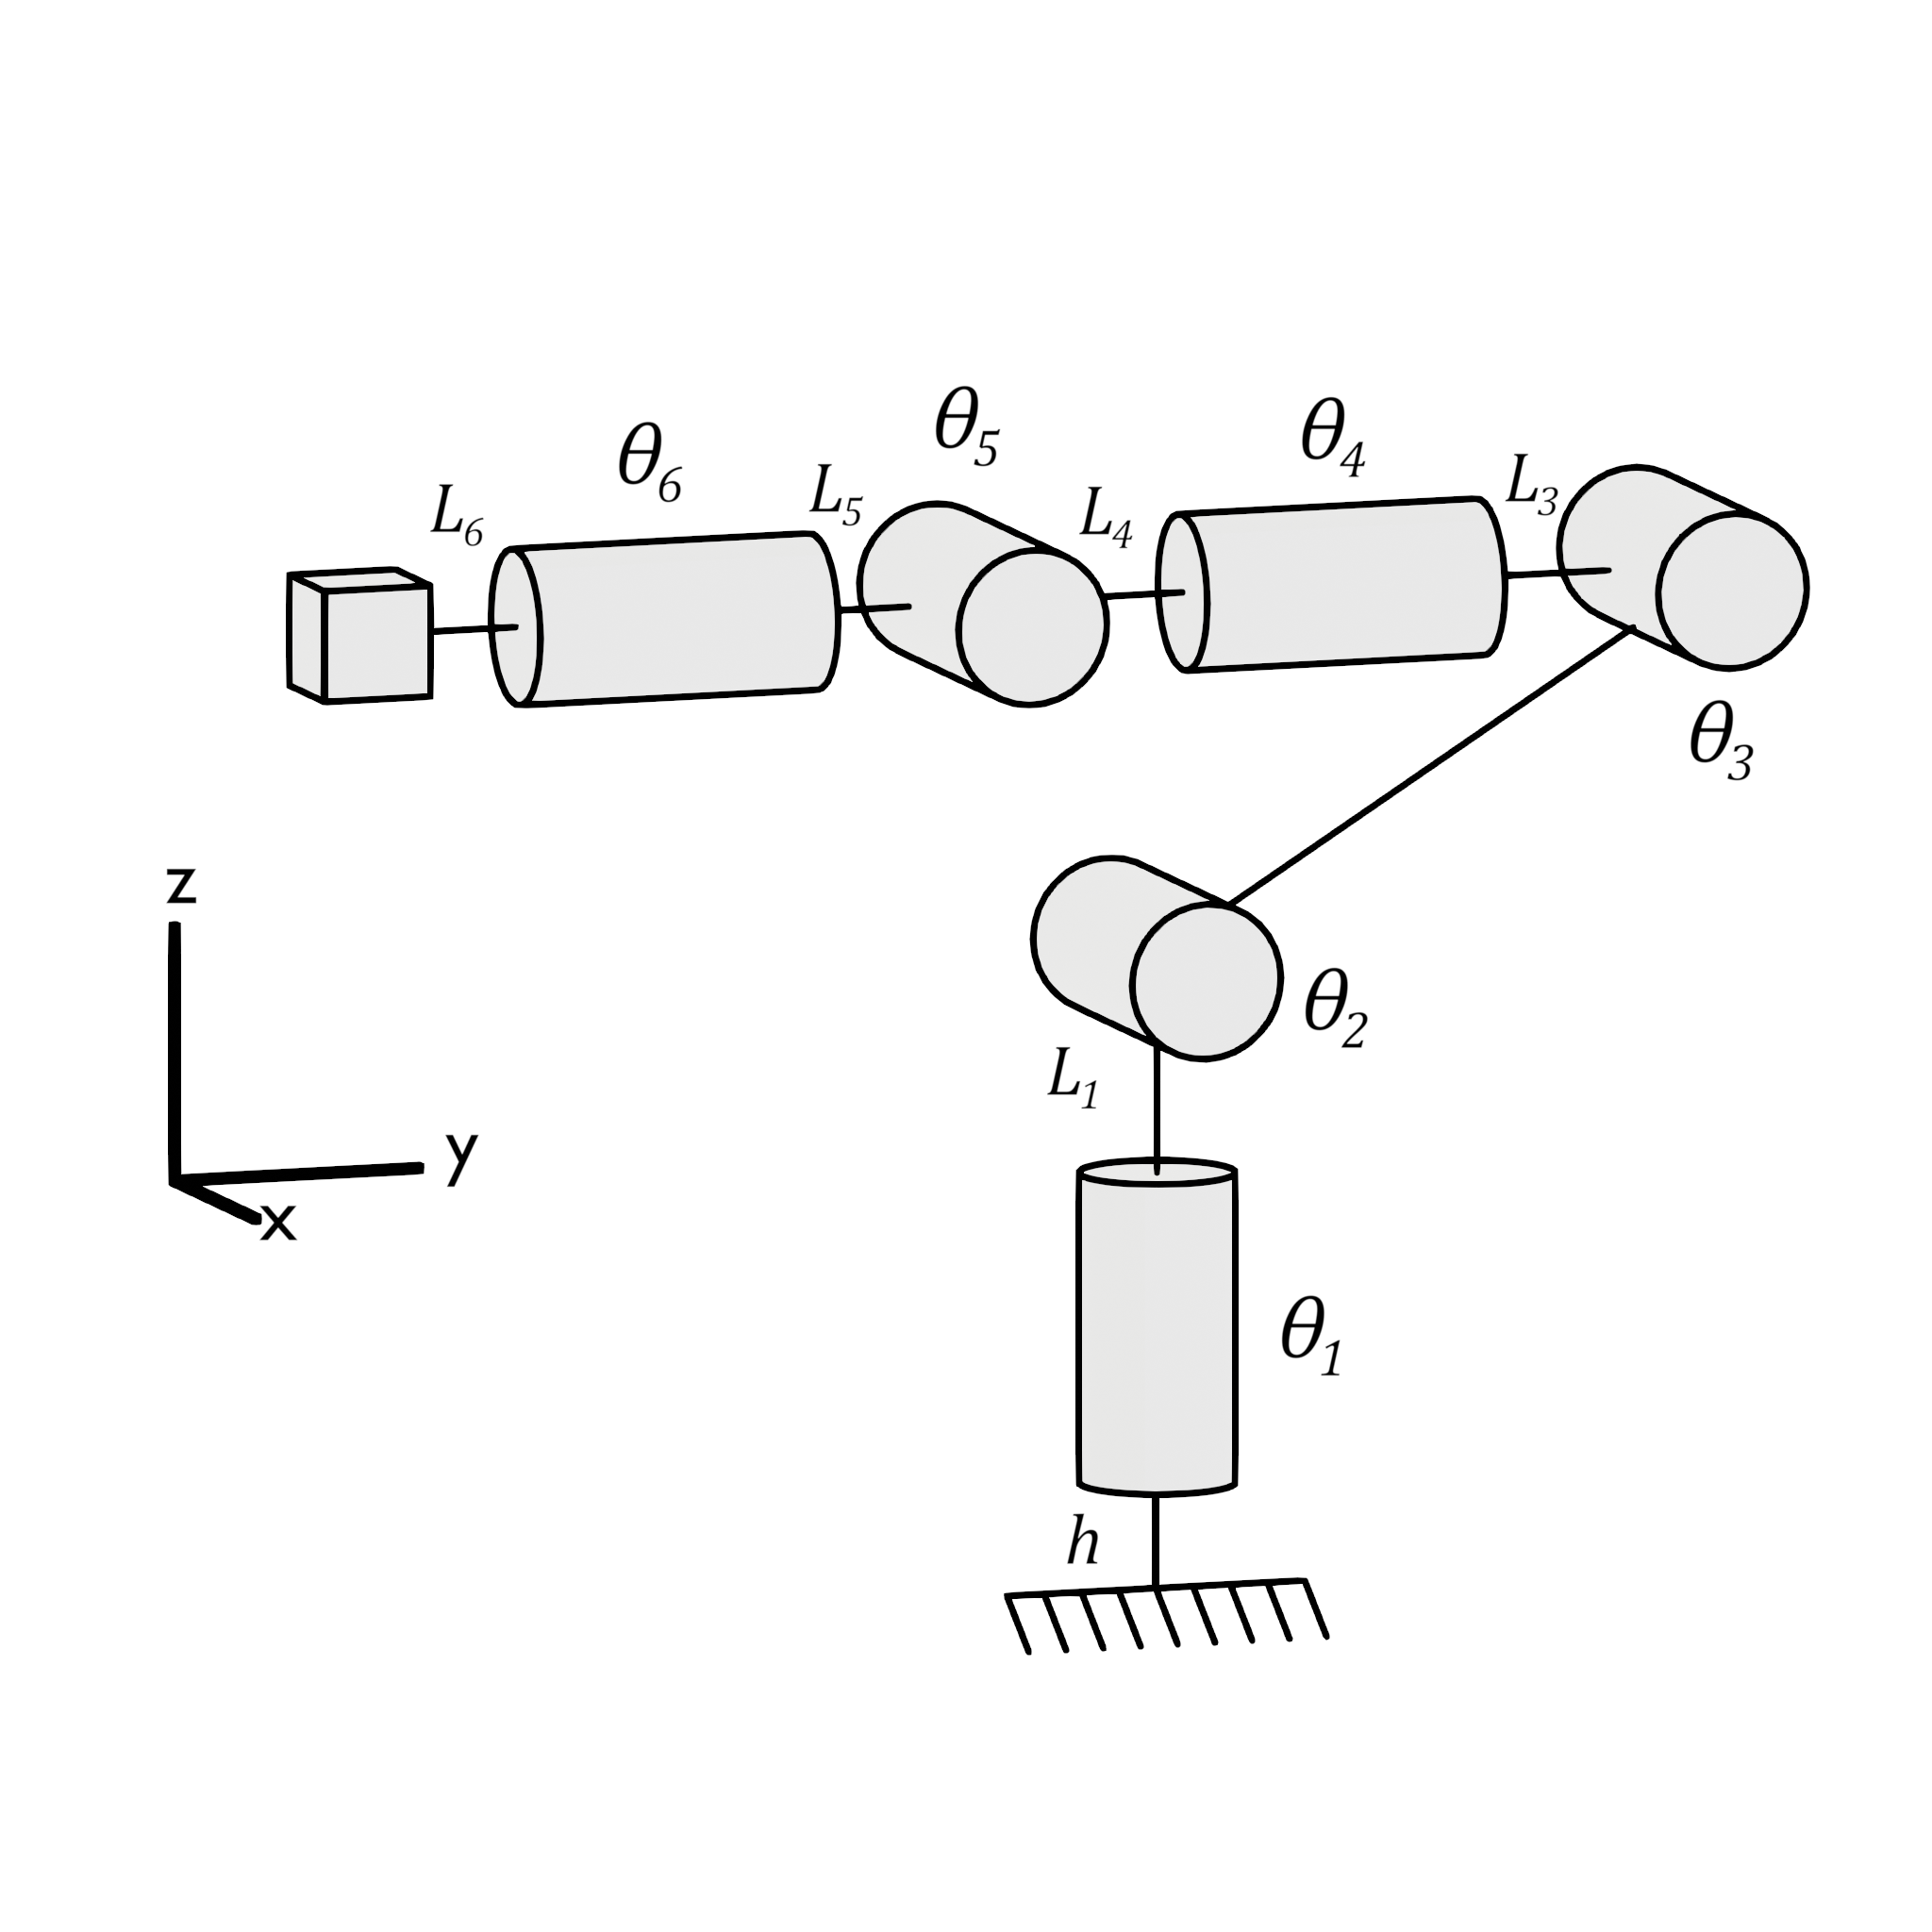
\includegraphics[width=0.7\linewidth]{img/mo6_joint-diagram.png} 
    \caption{Joint diagram of the Mo-6 robot.}
    \label{fig:joint_diagram}
\end{figure}

Figure~\ref{fig:joint_diagram} shows the joints of the Mo-6 robot. $\theta_{1}$, $\theta_{2}$, and $\theta_{3}$ comprise the positioning joints; $\theta_{4}$, $\theta_{5}$, and $\theta_{6}$ comprise the orienting joints, constructed in the spherical wrist configuration.

\begin{figure}[h!]
    \centering
    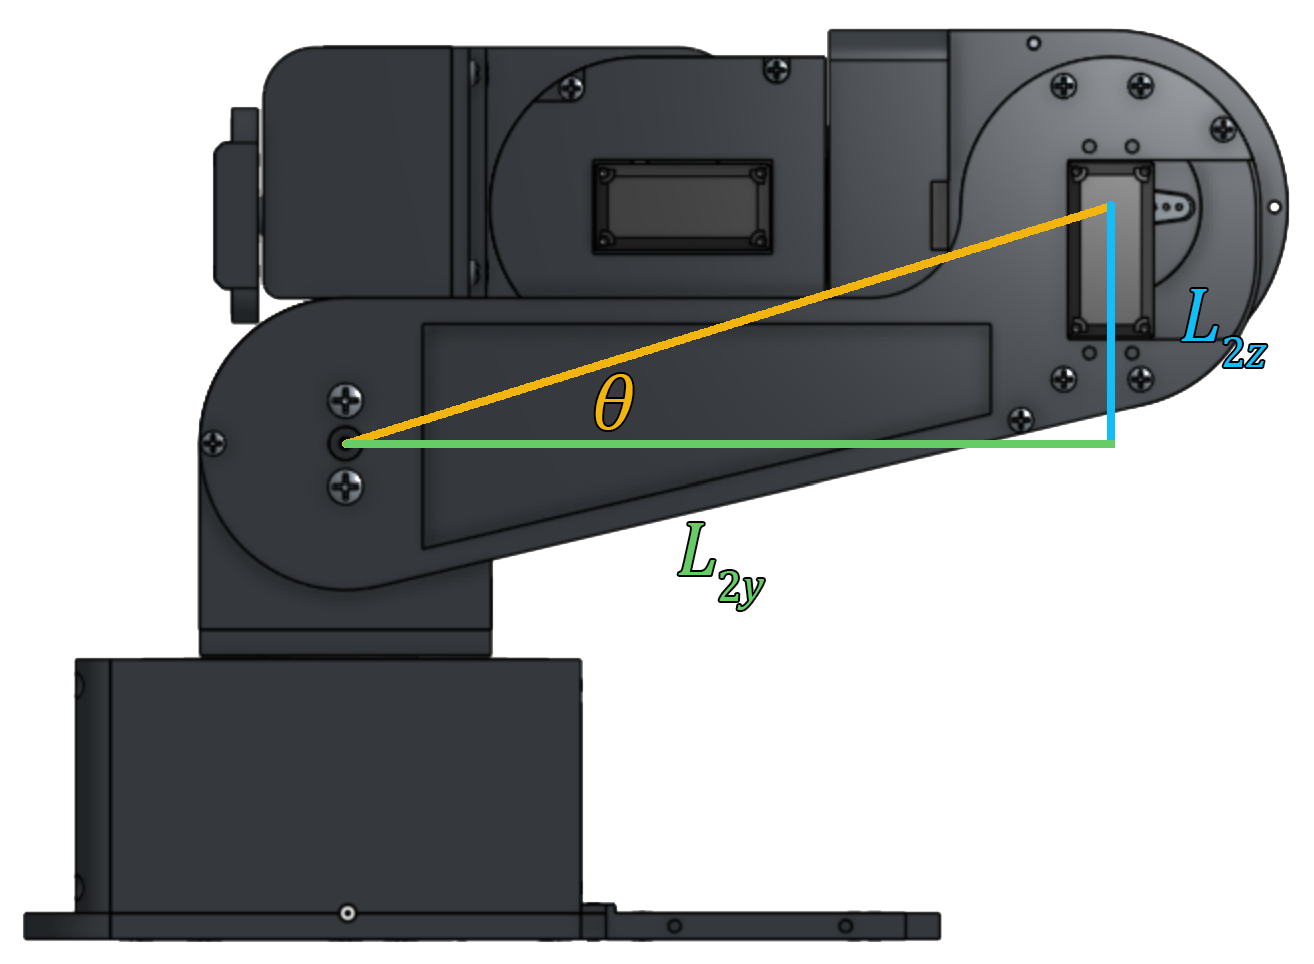
\includegraphics[width=0.65\linewidth]{img/mo6_link2-offset.png} 
    \caption{Diagram of $y$-axis and $z$-axis offset distances between joint 2 and joint 3.}
    \label{fig:j2_j3_offset}
\end{figure}

The only notable deviation from this structure on the Mo-6 is that when the robot is in its rest position, there is an angled offset between joint 2 and joint 3. This can be seen in Figure~\ref{fig:j2_j3_offset}, which shows a side view of Mo-6 with the aesthetic shell of its second link removed. The offset has been marked with distances $L_{2y}$ and $L_{2z}$, and $\theta$ as the resulting offset angle. As such, any kinematic models of the robot must take into account this offset. All other joints are collinear and/or coaxial where relevant.

\subsubsection{Forward Kinematics}

The forward kinematics of Mo-6 can be defined using the Power of Exponentials formula discussed by Lynch and Park in Modern Robotics, \cite{modernrobotics}.

As per Figure~\ref{fig:joint_diagram}, define:
\begin{itemize}
    \item $h$ as the distance between the ground and $\theta_{1}$;
    \item $L_{1}$ as the distance between $\theta_{1}$ and $\theta_{2}$;
    \item $L_{3}$ as the distance between $\theta_{3}$ and $\theta_{4}$;
    \item $L_{4}$ as the distance between $\theta_{4}$ and $\theta_{5}$;
    \item $L_{5}$ as the distance between $\theta_{5}$ and $\theta_{6}$;
    \item and $L_{6}$ as the distance between $\theta_{6}$ the end-effector.
\end{itemize}
$L_{2}$ is defined as the components $L_{2y}$ and $L_{2z}$, as per Figure~\ref{fig:j2_j3_offset}. Screw axes $\mathcal{S}_{n}$ can then be defined for each joint as follows:
\begin{align*}
    \mathcal{S}_{1} = \begin{bmatrix}
    0 \\ 0 \\ 1 \\ 0 \\ 0 \\ h    
    \end{bmatrix}, \quad
    \mathcal{S}_{2} = \begin{bmatrix}
    1 \\ 0 \\ 0 \\ 0 \\ 0 \\ h + L_{1}   
    \end{bmatrix}, \quad
    \mathcal{S}_{3} = \begin{bmatrix}
    1 \\ 0 \\ 0 \\ 0 \\ -L_{2y} \\ h + L_{1} + L_{2z}   
    \end{bmatrix}
\end{align*}

\begin{align*}
    \mathcal{S}_{4} = \begin{bmatrix}
    0 \\ -1 \\ 0 \\ 0 \\ -L_{2y} + L_{3} \\ h + L_{1} + L_{2z}
    \end{bmatrix}, \quad
    \mathcal{S}_{5} = \begin{bmatrix}
    1 \\ 0 \\ 0 \\ 0 \\ -L_{2y} + L_{3} + L_{4} \\ h + L_{1} + L_{2z}
    \end{bmatrix}, \quad
    \mathcal{S}_{6} = \begin{bmatrix}
    0 \\ -1 \\ 0 \\ 0 \\ -L_{2y} + L_{3} + L_{4} + L_{5} \\ h + L_{1} + L_{2z}
    \end{bmatrix}
\end{align*}

and the end-effector transformation at rest, $M$ can be defined as
\begin{align*}
    M = \begin{bmatrix}
        1 & 0 & 0 & 0 \\
        0 & 1 & 0 & -L_{2y} + L_{3} + L_{4} + L_{5} + L_{6} \\
        0 & 0 & 1 & h + L_{1} + L_{2z} \\
        0 & 0 & 0 & 1 \\
    \end{bmatrix} \in SE(3)
\end{align*}

which can be used in the PoE formula:
\begin{align}\label{eq:poe_formula}
    T(\theta) &= 
    e^{\displaystyle [\mathcal{S}_{1}]\theta_{1}}
    e^{\displaystyle [\mathcal{S}_{2}]\theta_{2}}
    e^{\displaystyle [\mathcal{S}_{3}]\theta_{3}}
    e^{\displaystyle [\mathcal{S}_{4}]\theta_{4}}
    e^{\displaystyle [\mathcal{S}_{5}]\theta_{5}}
    e^{\displaystyle [\mathcal{S}_{6}]\theta_{6}}
    M \in SE(3),\\
    \theta &= \begin{bmatrix}
        \theta_{1} & \theta_{2} & \theta_{3} & \theta_{4} & \theta_{5} & \theta_{6} 
    \end{bmatrix}^{T} \in \mathbb{R}^{6} \nonumber
\end{align}

\begin{table}[htbp]
    \centering
    \caption{Physical values for PoE parameters.}
    \label{tab:poe_values}
    \begin{tabular}{|l|l|}
        \hline
        \textbf{Parameter} & \textbf{Value (mm)} \\
        \hline
        $h$ & 65.35 \\
        $L_{1}$ & 50.30 \\
        $L_{2y}$ & 179.00 \\
        $L_{2z}$ & 55.30 \\
        $L_{3}$ & 65.85 \\
        $L_{4}$ & 44.30 \\
        $L_{5}$ & 88.00 \\
        $L_{6}$ & (Decided by chosen end-effector) \\
        \hline
    \end{tabular}
\end{table}

Table~\ref{tab:poe_values} shows the physical values of the parameters used in Equation~\ref{eq:poe_formula}.

\subsubsection{Workspace \& Joint Limits}

\begin{table}[htbp]
    \centering
    \caption{Joint angle limits, listed with reference axis taken as $0^{\circ}$.}
    \label{tab:joint_limits}
    \begin{tabular}{|l|l|l|l|}
        \hline
        \textbf{Joint} & Reference Axis & Limit ($^{\circ}$) & Rest Position ($^{\circ}$) \\
        \hline
        $\theta_{1}$ & $x$ & $180^{\circ}$\footnotemark & $90^{\circ}$ \\
        $\theta_{2}$ & $y$ & $180^{\circ}$\footref{fn:270_servo} & $0^{\circ}$ \\
        $\theta_{3}$ & $-y$ & $180^{\circ}$ & $0^{\circ}$ \\
        $\theta_{4}$ & $-x$ & $180^{\circ}$ & $90^{\circ}$ \\
        $\theta_{5}$ & $-z$ & $180^{\circ}$ & $90^{\circ}$ \\
        $\theta_{6}$ & $x$ & $180^{\circ}$ & $90^{\circ}$ \\
        \hline
    \end{tabular}
\end{table}
\footnotetext{Technically, $\theta_{1}$ and $\theta_{2}$ both use the Miuzei MS24 20kg Digital Servo, which has an angle range of $270^{\circ}$, however for consistency, ease of use, and to simplify the construction, the servo has simply been taken as having the same $180^{\circ}$ limit as the MG996R servos used in the other joints.\label{fn:270_servo}}

As the robot is constructed using servos for actuation, the joints are not continuous and have specific limits. These can be seen in Table~\ref{tab:joint_limits}. The reference axes and subsequent rest positions for each joint are based on the servos themselves rather than the mathematical model of Equation~\ref{eq:poe_formula}. The reference axes are defined as per the axes shown in Figure~\ref{fig:joint_diagram}.

% --- DESIGN & ASSEMBLY -------------------------------------------------------------------------------------
\newpage
\subsection{Design}


% --- BIBLIOGRAPHY ---------------------------------------------------------------------------------
\newpage
\printbibliography

\end{document}